\documentclass[10pt]{article}

\usepackage[margin=1.5cm, includefoot, footskip=30pt]{geometry}

\usepackage{amssymb}
\usepackage{amsmath}
\usepackage{amsthm}
\usepackage{booktabs}
\usepackage{caption}
 \usepackage{epsfig}
\usepackage{graphicx}
\usepackage{hyperref}
\usepackage{psfrag}
\usepackage{subcaption}
\usepackage{ulem}
\usepackage{standalone}
\usepackage{tikz}

\newcommand{\rd}{\mathrm{d}}
\newcommand{\be}{\begin{eqnarray}}
\newcommand{\ee}{\end{eqnarray}}
\usepackage{tabularx} % http://ctan.org/pkg/tabularx
\renewcommand{\arraystretch}{1.5} % tables have longer cells

\newtheorem{theorem}{Theorem}

% \journal{Undecided Journal}

\title{An evolutionary game theory model for devaluing rhinos}
\author{Nikoleta E. Glynatsi, Vincent Knight, Tamsin E. Lee} %TODO Authors
\date{}

\begin{document}

\maketitle

\begin{abstract}

Rhino poaching has escalated in recent years due the demand for rhino horn in 
Asian countries. Rhino horn is used in Traditional Chinese Medicine and as a 
status symbol of success and wealth. Wild life managers attempt to minimise
the rhino casualties with approaches such as devaluation of the rhino horn. 
The  most common strategy of devaluing horns includes dehorning. In~\cite{Lee}
game theory modelling was used to examined the interaction of poachers and
wild life managers.  A manager can either `dehorn' their rhinos or leave the
horn attached. Poachers may chose to to behave `selectively' or `indiscriminately'.
The approach described in this paper builds upon~\cite{Lee} and investigates 
the interactions  between the poachers using evolutionary game theory. 
Evolutionary game theory, allows us to explore the evolutionary stabilities 
of the strategies available to a poacher. The purpose of this work is to discover
whether conditions which encourages the poachers to behave selectively,
they only kill those rhinos with full horns, exist. Notwithstanding, the 
analytical results prove that poachers will never adopt a selective behaviour
as long as there is the slightest gain from a partial horn. Additionally, poachers
behaving indiscriminate can be proven to be stable and robust. Thus, we 
conclude that dehorning is not the dominant strategy for a wild life manager,
and we suggest that money are spend on security.

\end{abstract}

%=============================================
\section{Introduction}\label{section:introduction}

The illegal trade in rhino horn supports aggressive poaching syndicates and a 
black market~\cite{Nowell1992}. This lucrative market entices people to invest
their time and energy to gain a `winfall' in the form of a rhino horn, through the 
poaching of rhinos. In recent years poaching has escalated to an unpresidented 
level resulting in concerns over their future existence~\cite{Smith1993}. In 
response, rhino conservation has seen increased  ilitarisation with `boots on the 
ground' and `eyes in the sky'~\cite{duffy_st}. An alternative method is to 
devalue the horn itself, one of the main  methods being the removal so that only
a stub is left. The first attempt at large-scale rhino dehorning as an anti-poaching
measure was in Damordond,  Namibia, in 1989~\cite{Milner1992}. Other methods
of devaluing the horn that have been suggested include
the insertion of poisons, dyes or GPS trackers~\cite{Gill2010,Smith1993}. However, 
like dehorning, they cannot remove all the potential gain from an intact horn 
(poison and dyes fade or GPS trackers can be removed). This paper builds on 
the work of~\cite{Lee} and considers the general strategy of devaluing horns,
which includes dehorning.

Rhino populations now persist largely in protected areas or on private land, and
require intensive protection~\cite{Ferreira2014}. For wildlife managers law 
enforcement is often one of the main methods of deterring poaching, however 
rhino managers can remove the poaching incentive by devaluing their rhinos 
\cite{Milner1992}. In~\cite{Milner1992} they found the 
optimum proportion to dehorn using mean horn length as a measure of the 
proportion of rhinos dehorned. They showed, with realistic parameter values, 
that the optimal strategy is to dehorn as many rhinos as possible. 
A manager does not need to choose between law enforcement or devaluing, but
perhaps adopt a combination of the two; especially given that devaluing rhinos 
comes at a cost to the manager, and the process comes with a risk to the rhinos.

A recent paper modelled the interaction between a rhino manager and poachers
using game theory~\cite{Lee}.  The authors consider a working year of a single 
rhino manager.  A manager is assumed to have standard yearly resources which
can be allocated on devaluing a proportion of their rhinos or spent on security. 
It is assumed that all rhinos initially have intact horns. Poachers may either only
kill rhinos with full horns, `selective poachers', or kill all rhinos they encounter, 
`indiscriminate poachers'. If all rhinos are left by the rhino manager with their 
intact horns, it does not pay poachers to be selective so they will chose to be 
indiscriminate. Conversely, if all poachers are selective, it pays rhino managers 
to invest in devaluing their rhinos. This dynamic is represented in Fig.~\ref{fig:RhinoPic}.
Assuming poachers and managers will always behave so as to maximise their 
payoff, there are two equilibriums: either all devalued and all poachers selective;
or all horns intact and all poachers indiscriminate. Essentially, either the managers 
win, the top left quadrant of Fig.~\ref{fig:RhinoPic}, or the poachers win, the bottom
right quadrant of Fig.~\ref{fig:RhinoPic}. The paper concludes that poachers will
always choose to behave indiscriminately, and thus the game settles to the top
left quadrant, i.e., the poachers win.

\begin{figure}[!htbp]
    \centering
    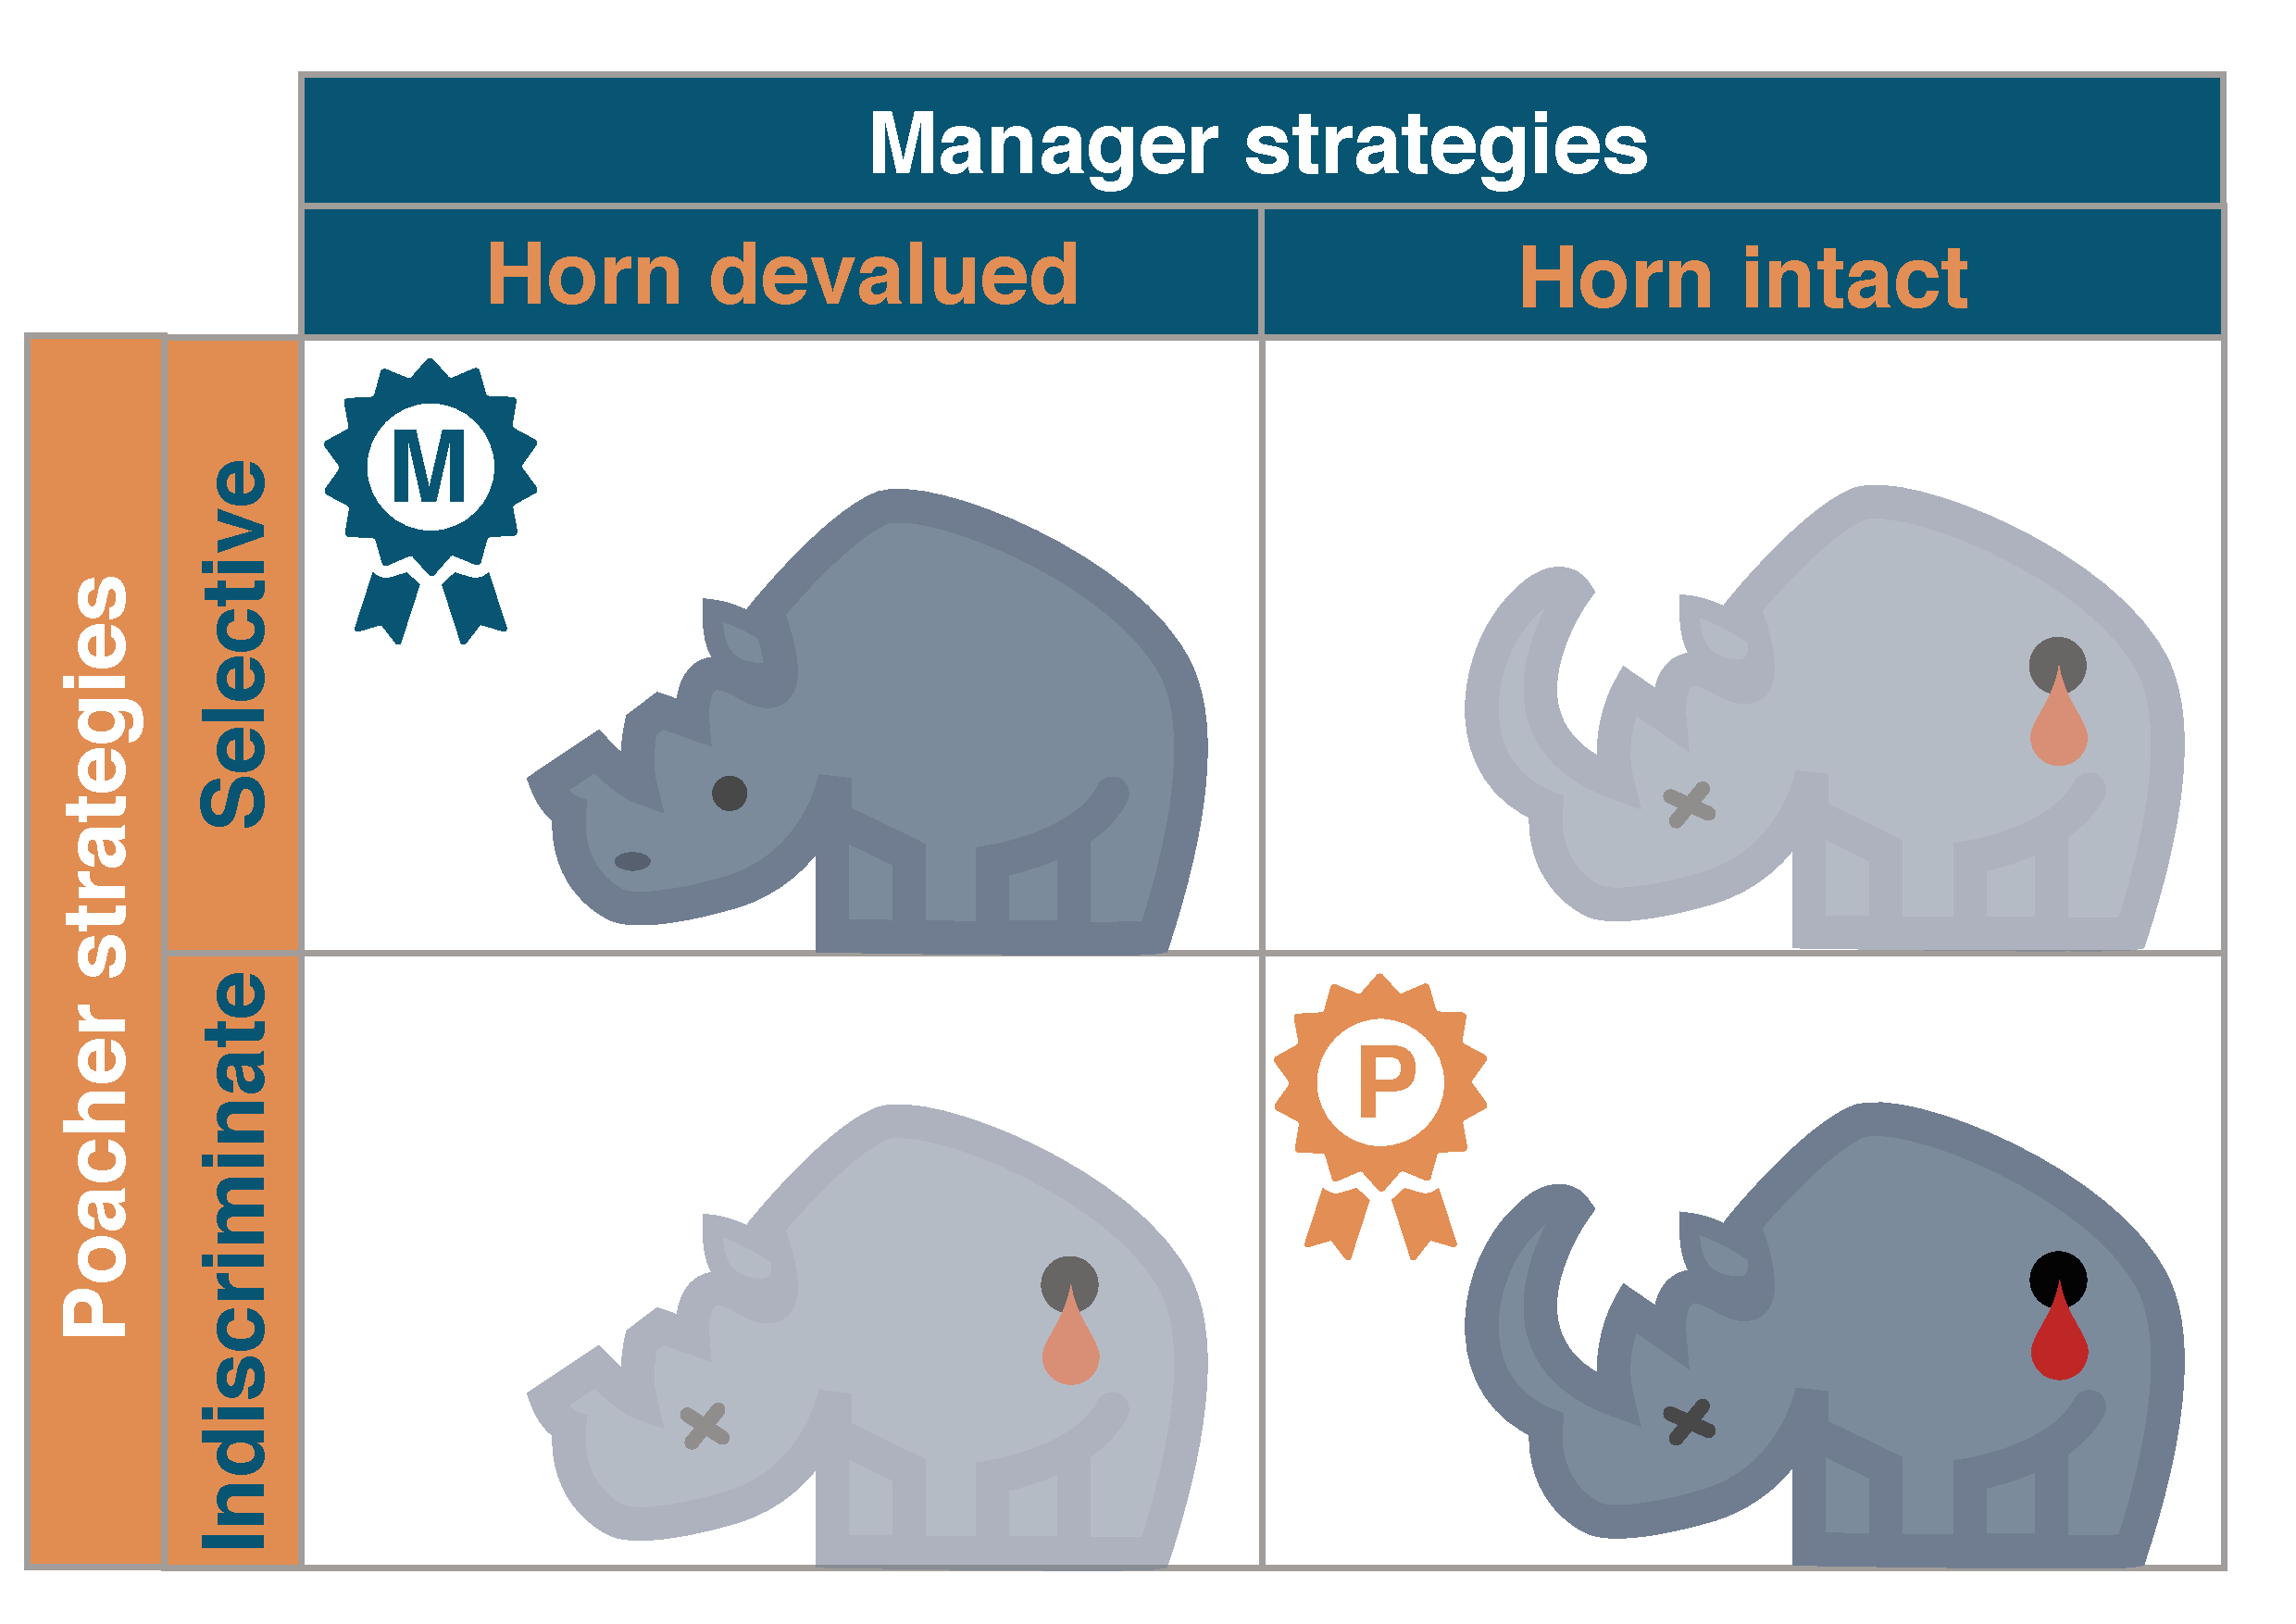
\includegraphics[scale=0.2]{images/RhinoPic.pdf}
    \caption{\label{fig:RhinoPic} The game between rhino manager and rhino 
    poachers. The system settles to one of two equilibriums, either devaluing is effective or not.}
\end{figure}

The work of~\cite{Lee} did not take in to account the population dynamic effect
of  these strategies. In a population full of selective poachers would their be 
a benefit to a single poacher becoming indiscriminate or vice versa? This notion 
is explored here using evolutionary game theory~\cite{Smith}. The 
game is not that of two players anymore (manager and poacher) but an infinite
population of poachers is considered. This allows for the interaction between poachers
over multiple plays of the game to be explored with the rhino manager being the
one that creates the conditions of the population. 

In evolutionary game theory, we assume infinite populations and in our
model this will be represented by \(\chi=(x_1, x_2)\) with \(x_1\) proportion of the
population using a strategy of the first type and \(x_2\) of the second, denoted
by \(s_1, s_2\) respectively. We assume there is a utility function \(u_1\) and 
\(u_2\) that maps the population to a fitness for each type,

\[ u_1(\chi)  \qquad u_2(\chi).\] 

In evolutionary game theory these utilities are used to dictate the evolution of
the population over time, according to the following differential equations,

\begin{eqnarray}
    \label{eqn:u_differential_eq}
    \left\{
    \begin{array}{cl}
    \dfrac{dx_1}{dt}=x_1(u_1(\chi)-\phi),
    \\
    \\
    \dfrac{dx_2}{dt}= x_2(u_2(\chi)-\phi).
    \end{array} \right.
\end{eqnarray}

The overall population is assumed to remain stable thus, \(x_1 + x_2 = 1 \)
and

\begin{eqnarray}
    \dfrac{dx_1}{dt}  + \dfrac{dx_2}{dt} = 0 \Rightarrow x_1(u_1(\chi) - \phi)
     + x_2(u_2(\chi) - \phi)=0.
\end{eqnarray} 

Thus the average fitness can be written as,

\begin{eqnarray}
\label{eqn:average_fitness}
    \phi=x_1u_1(\chi) + x_2u_2(\chi).
\end{eqnarray}

By substituting (\ref{eqn:average_fitness}) and \(x_2= 1 - x_1\) 
in (\ref{eqn:u_differential_eq}),

\begin{eqnarray}
    \label{eqn:u_differential_simplified}
    \frac{dx_1}{dt}= x_1(1 - x_1)(u_1(\chi) - u_2(\chi)).
\end{eqnarray}

The equilibria of the differential equation (\ref{eqn:u_differential_simplified})
are given by, \(x_1=0\), \(x_1=1\), and \(0<x_1<1 \mbox{ for } u_1(\chi)=u_2(\chi)\).

These equilibria correspond to stability of the population: the differential 
equation (~\ref{eqn:u_differential_simplified}) no longer changes. Further to
this, evolutionary game theory aims to qualify these equilibria subject to 
evolutionary changes.

The notion of evolutionary stability can be checked only for the stable strategies.
For a stable strategy to be an Evolutionary Stable Strategy (ESS) it must remain 
the best response even in a mutated population \(\chi_\epsilon\). A mutated population 
is called the post entry population, 
where a small proportion \(\epsilon\) starts deviating and adopts a different strategy.
Fig.~\ref{fig:stable_ess_driagrams} illustrates two potential strategies: without 
outside stimulation neither marble would move. In Fig.~\ref{fig:ess_diagram}
however the stability can be described as "stronger": with a small nudge the marble
would return to its stable position. In Fig.~\ref{fig:stable_diagram} any non zero
nudge would move the marble out of its equilibria.

\begin{figure}[!htbp]
\begin{center}
    \begin{subfigure}{0.40\textwidth}
    \includestandalone[width =\textwidth]{images/stable}
    \caption{\label{fig:stable_diagram} A diagram of a stable strategy which 
    is not ESS.}
    \end{subfigure}
    \begin{subfigure}{0.40\textwidth}
    \includestandalone[width = \textwidth]{images/evolutionary_stability}
    \caption{\label{fig:ess_diagram}A diagram of a stable strategy which is ESS.}
    \end{subfigure}
        \caption{\label{fig:stable_ess_driagrams} Diagrams of stable strategies.}
\end{center}
\end{figure}

In Section~\ref{section:the_model}, we determine expressions
for \(u_1, u_2\) that correspond to a population of wild rhino poachers and we
explore the stability of the equilibria identified in~\cite{Lee}. The results
contained in this paper are proven analytically, and more specifically it is 
shown that:

\begin{itemize}
    \item all poachers behaving selectively is trivially unstable,  
    \item a mixed population where selective and indiscriminate poachers
          learn to co exist can not hold in sensible scenarios,
    \item all poachers adopting an indiscriminate strategy is an evolutionary 
          stable strategy.
\end{itemize}

This implies that under almost all conditions, no matter what current proportion 
of
of poachers are acting selectively, the population will eventually turn in to a 
population of only indiscriminate poachers.

%============================================================
\section{The Utility Model}\label{section:the_model}

As discussed briefly in Section~\ref{section:introduction}, a wild rhino poacher
can adopt two strategies, to either behave selectively
or indiscriminately. Calculating the utility for each strategy, the gain and cost
that poachers are exposed to must be taken into account. The poacher incurs a
loss from seeking a rhino, and the risk involved. The gain depends upon the value
of horn, the proportion of horn remaining after the manager has devalued the 
rhino horn and the number of rhinos (devalued and not).

Let us first consider the gain to the poacher, where \(\theta\) is the amount of 
horn taken. We assume rhino horn value is determined by weight only, a 
reasonable assumption as rhino horn is sold in a grounded form~\cite{Saverhino}.
Referring to Fig.~\ref{fig:RhinoPic}, clearly if the horn is intact, the amount of
horn gained is \(\theta=1\) for both the selective and the indiscriminate poacher.
If the rhino horn has been devalued, and the poacher is selective, the amount of horn 
gained is \(\theta=0\) as the poacher does not kill. However, if the poacher is 
behaving indiscriminately, the amount of horn gained is \(\theta = \theta_r\)
(for some \(0<\theta_r<1\)). 
Therefore, the amount of horn gained in the general case is

\begin{eqnarray}
    \label{eqn:theta}
    \theta(r, s) = s (1 - r) + (1 - s) ((\theta_r - 1) r + 1),
\end{eqnarray}

where \(r\) is the proportion of rhinos that have been devalued, and \(s\) is the 
proportion of selective poachers. Note that since \(\theta_r, r, s  \in [0, 1]\), then
\(\theta(r, s) > 0\). Standard supply and demand arguments imply that the value
of rhino horn decreases as the quantity of horn increases~\cite{mankiw2010}.
Thus at any given time the expected gain for a poacher is

\begin{eqnarray}
    \label{eqn:individual_gain}
    H \theta(r,s)^{-\alpha},
\end{eqnarray}

where \(H\) is a scaling factor associated with the value of a full horn, and 
\(\alpha \geq 0\) is a constant that determines the precise relationship between
the quantity and value of the horn.  Fig.~\ref{fig:GainCurve}, verifies that the 
gain curve corresponds to a demand curve.

\begin{figure}[!htbp]
\centering
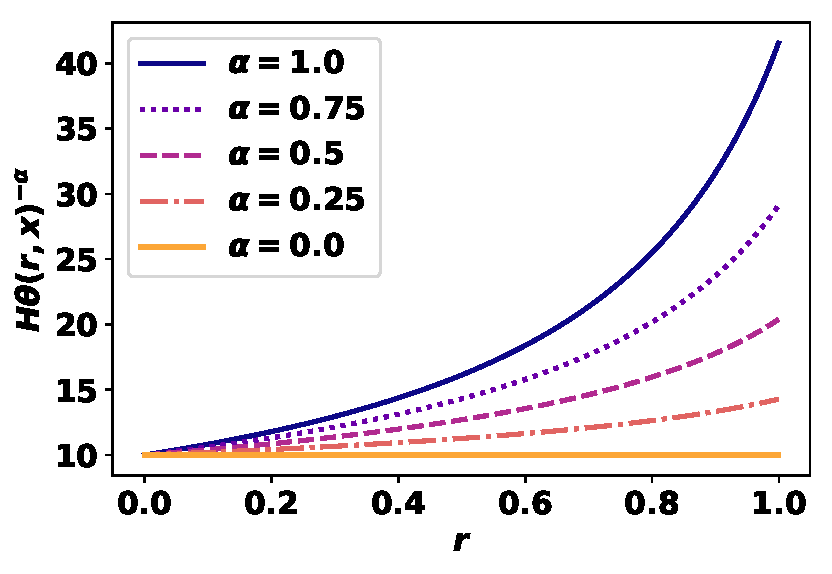
\includegraphics[width=0.4\textwidth]{images/gain_curve.pdf}
\caption{\label{fig:GainCurve} \(H \theta(r, s) ^{- \alpha}\) for values 
\(H = 10, \theta_r = 0.3\) and \(s = 0.2.\).}
\end{figure}

An individual interacts with the population, denoted as \(\chi=(x, 1 -x )\). Thus,
the gain is either

\begin{eqnarray}
    \label{eqn:gain}
    \left\{
    \begin{array}{cl}
    \theta(r, 1) H \theta(r, x)^{-\alpha} & \mbox{ selective poacher}
    \\
    \theta(r, 0) H \theta(r, x)^{-\alpha} & \mbox{ indiscriminate poacher}
    \end{array} \right.
\end{eqnarray}

depending on the chosen strategy of the individual, see Fig.~\ref{fig:RhinoPic}.

Secondly we consider the costs incurred by the poacher. Let us denote the number
of rhinos that will be considered at risk given \(r\) and \(s\) as \(\phi(r,s)\).
The rhinos \textbf{not} at risk are the devalued ones 
that cross the paths of selective poachers. Thus:

\begin{eqnarray}
    \label{eqn:psi}
    \psi(r, s) = 1 - rs.
\end{eqnarray}

Additionally, the poachers are also exposed to a risk. The risk to the poacher is
the opposite of the proportion of rhinos devalued \(r\), since the rhino manager
can spend more on security if the cost of devaluing is low.

\begin{eqnarray}
    \label{eqn:risk}
    (1 - r)^{\beta},
\end{eqnarray}

where \(\beta \geq 0\) is a constant that determines the precise relationship between
the proportion of rhinos not devalued and the security on the grounds. Therefore,
at any given time the expected cost for a poacher is, 

\begin{eqnarray}
    \label{eqn:individual_cost}
    \begin{array}{l}
    F \psi(r, s)^{\gamma} (1 - r)^{\beta} = F (1 - rs) ^{\gamma} (1 - r) ^{\beta}
    \end{array}
\end{eqnarray}

where \(F\) and \(\gamma \geq 0\) are constants that determine the precise relationship
between the proportion of vulnerable rhinos and the probability of finding a rhino,
such that \(\gamma\) close to zero indicates very sparse rhinos. Fig.
\ref{fig:CostCurves},  verifies the decreasing relationship between \(r\) and the
cost.

\begin{figure}[!htbp]
\begin{center}
    \begin{subfigure}{0.40\textwidth}
        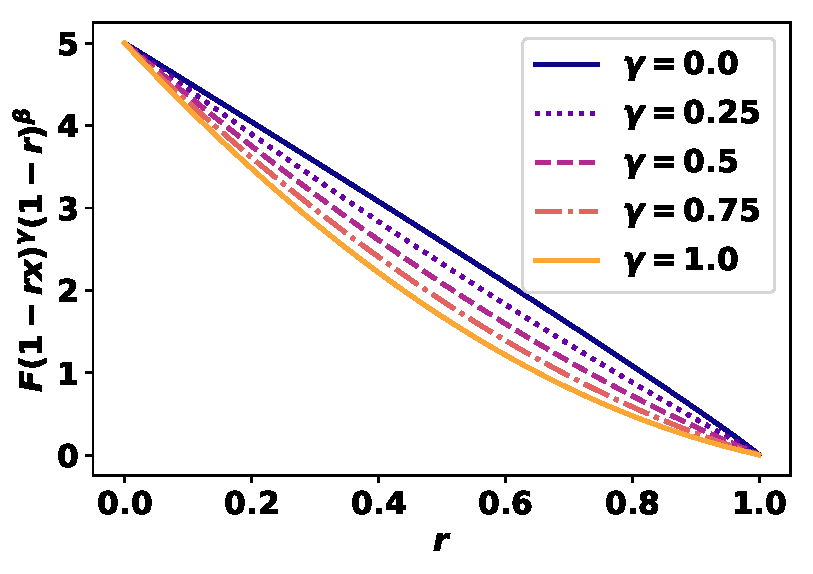
\includegraphics[width=\linewidth]{images/gammas_curve.pdf}
        \caption{For values, \(s=0.7, F=5\) and \(\beta=0.95\).}
    \end{subfigure}
    \begin{subfigure}{0.40\textwidth}
        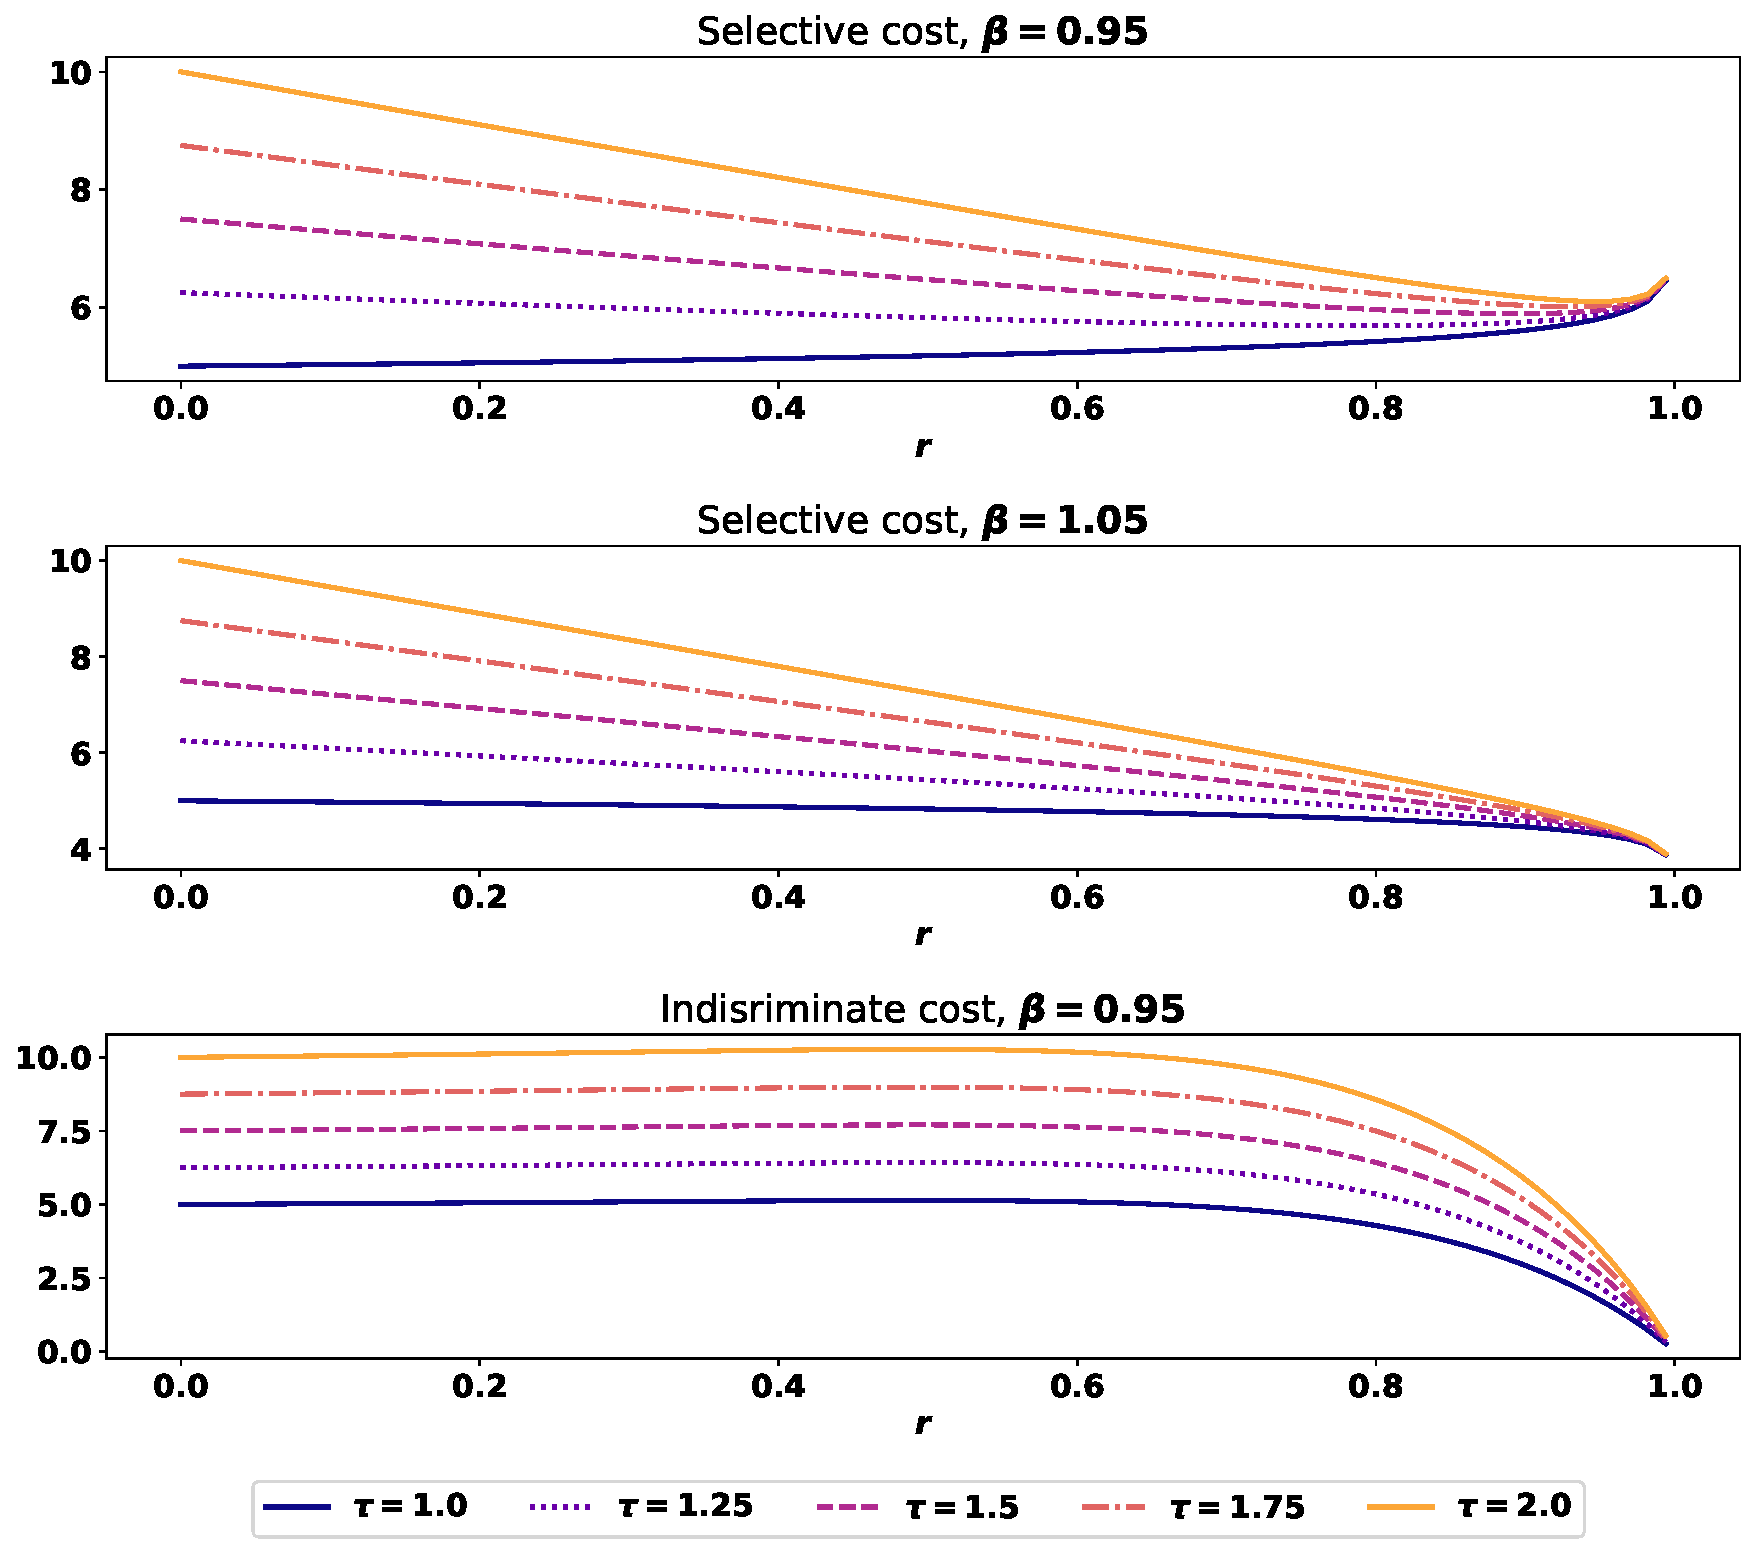
\includegraphics[width=\linewidth]{images/betas_curve.pdf}
        \caption{For values, \(s=1, F=5\) and \(\gamma=0.95\).}
    \end{subfigure}
\caption{\(F (1 - rs)^{\gamma} (1 - r)^{\beta}\).}\label{fig:CostCurves}
\end{center}
\end{figure}

Note that for a indiscriminate poachers \(s = 0\) the seeking 
cost (\ref{eqn:risk}) will always be \(1\), thus the cost of finding a rhino is greater
than the same cost for a selective poacher. However, a selective poacher needs 
more time to secure an `available' rhino, if they exist at all. Hence, an 
additional cost that tends to infinity as \(r \rightarrow 1\) must be applied, 

\begin{eqnarray}
    \label{eqn:selective_cost}
    \left\{
    \begin{array}{cl}
    \frac{1}{\psi(r, 1)} = \frac{1}{1 - r} & \mbox{ selective poacher}
    \\
    \frac{1}{\psi(r, 0)} = 1 & \mbox{ indiscriminate poacher}
    \end{array} \right.
\end{eqnarray}

To summarise, the cost incurred by a given individual when interacting with
the population is given by 

\begin{eqnarray}
    \label{eqn:cost}
    \left\{
    \begin{array}{cl}
    \frac{1}{1 - r}  F(1- rx)^{\gamma} (1-r)^{\beta}& \mbox{ selective poacher}
    \\
    F(1 - rx)^{\gamma} (1-r)^{\beta}& \mbox{ indiscriminate poacher}
    \end{array} \right.
\end{eqnarray}

As a result, the utility of the poachers can now be defined. Let \(\sigma = (s, 1 - s)\)
denote the strategy of an individual. Thus \(\sigma = (1, 0)\) represent an
individual poacher who is selective and \(\sigma = (0, 1)\) represent an individual
poacher who is indiscriminate. Combining~(\ref{eqn:gain}) and (\ref{eqn:cost})
gives the utility function for the individual poacher \(\sigma\) in the population
\(\chi\),

\begin{eqnarray}
\label{eqn:utility}
u(\sigma, \chi) = s u_1(\chi) +(1 - s) u_2(\chi),
\end{eqnarray}
where

\begin{eqnarray}
\label{eqn:USchi}
u_1(\chi) &=& \theta(r,1) H \theta(r,x)^{-\alpha}
- \frac{1}{1- r} F\psi(r, x)^{\gamma} (1-r)^{\beta} ,
\\
\label{eqn:UnotSchi}
u_2(\chi) &=& \theta(r,0) H \theta(r,x)^{-\alpha}
- F\psi(r, x)^{\gamma}  (1-r)^{\beta}.
\end{eqnarray}
Substituting~(\ref{eqn:USchi}) and~(\ref{eqn:UnotSchi}) into~(\ref{eqn:utility}) gives

\begin{eqnarray}
\label{eqn:tutility2}
u(\sigma, \chi) &=&
H (\theta_r r(1-s) - r + 1)\theta(r,x)^{-\alpha} - F\left(1-s + \frac{s}{1-r} \right)(1-rx)^{\gamma}(1-r)^{\beta} .
\end{eqnarray}

In Section~\ref{section:evolutionary_stability}, the notions of stability
and evolutionary stability of these two strategies as well as a potential 
mixed strategy will be investigated.

%=======================================================
\section{Evolutionary Stability}\label{section:evolutionary_stability}

By definition, for a strategy to be an ESS it must first be a best response to an 
environment where the entire population is playing the same strategy.
In our model there are three possible stable distributions based on the
equilibria of equation (\ref{eqn:u_differential_simplified}),

\begin{itemize} 
    \item All poachers are selective \(s=1\);
    \item All poachers are indiscriminate \(s=0\);
    \item Mixed population of selective and indiscriminate poachers.
\end{itemize}

Each of the equilibria will be examined in the following subsections.

\subsection{All poachers are selective \(s=1\)}

\begin{theorem}
Using the utility model descried in Section~\ref{section:the_model}, 
a population of selective poachers (\(\sigma=(1, 0)\)) is unstable.
\end{theorem}

\begin{proof}
    For \(\sigma=(1, 0)\) to be a best response to itself the utility of behaving 
    selectively in a population of selective poachers must be greater than the utility
    of a poacher behaving indiscriminately in a population of selective poachers,

    \begin{equation}
    u((1, 0),(1, 0)) > u((0, 1),(1, 0))
    \end{equation}
    
    where,
    
    \begin{eqnarray}
    \label{eqn:s1x1}
    u((1, 0),(1, 0)) = H(1 - r)^{1 - \alpha} - F(1 - r)^{\beta + \gamma - 1},
    \end{eqnarray}
    
    and 
    
    \begin{eqnarray}
    \label{eqn:s0x1}
    u((0, 1),(1, 0)) = H(\theta_r r +1 - r)(1 - r)^{-\alpha} - F(1 - r)^{\beta + \gamma} .
    \end{eqnarray}

    Setting~(\ref{eqn:s1x1}) to be greater than (\ref{eqn:s0x1}) gives the 
    condition,

    \begin{eqnarray}
    \label{eqn:s1x1_s0x1}
    H \theta_r r < F [1 - (1 - r)^{-1}](1 - r)^{\gamma + \beta + \alpha}
    \end{eqnarray}

    The left-hand size  will always be negative since \(1-(1-r)^{-1} \leq 0\)
    for any \(r\), on the other hand the right-hand side is always positive.
    Thus, (\ref{eqn:s1x1_s0x1}) can never hold.
\end{proof}

This implies that whilst~\cite{Lee} identified the individual poachers 
acting selectively as an equilibrium it is an extremely week equilibrium from 
the point of view of population stability: a slight change and the population 
will change.

\subsection{All poachers are indiscriminate \(s=0\)}

\begin{theorem}
Using the utility model descried in Section~\ref{section:the_model}, a population 
of indiscriminate poachers (\(\sigma=(0, 1)\)) is evolutionarily stable.
\end{theorem}

% \begin{theorem}
%   For \(\sigma=(0, 1)\) to be stable the utility of a poacher behaving 
%   indiscriminately in a population of indiscriminate poachers must be greater
%   than the utility of a poacher behaving selectively in a population of 
%   indiscriminate poachers,

%   \begin{equation}
%   u((0, 1),(0, 1)) > u((1, 0),(0, 1)),
%   \end{equation}

%   where,

%   \begin{eqnarray}
%   \label{eqn:s0x0}
%   u((0, 1), (0, 1)) = H(\theta_r r + 1 - r)(\theta_r r + 1 - r)^{-\alpha}  - F(1 - r)^{\beta},
%   \end{eqnarray}

%   and 

%   \begin{eqnarray}
%   \label{eqn:s1x0}
%   u((1, 0),(0, 1)) = H(1 - r)(\theta_r r + 1 - r)^{-\alpha} - F(1 - r)^{\beta-1}.
%   \end{eqnarray}

%   Setting~(\ref{eqn:s0x0}) to be greater than~(\ref{eqn:s1x0}) gives,

%   \begin{eqnarray}
%   \label{eqn:s0x0_s1x0}
%   H \theta_r r  > F [1 - (1 - r)^{-1}](1 - r)^{\beta}(\theta_r r - r + 1)^{\alpha}.
%   \end{eqnarray}

%   This inequality states that for indiscriminate behaviour to be stable, the value of
%   a partial rhino horn available needs to be greater than a given amount. 

%   Since \(1-(1-r)^{-1} \leq 0\), the righ-hand side of the inequality is always
%   negative where the left-hand side is always positive. Thus, inequality 
%   (\ref{eqn:s0x0_s1x0}) holds for any \(r\). So all indiscriminate
%   is proven to be stable.
% \end{theorem}

% Thereupon, the evolutionary stability of the strategy can now be explored. 

\begin{proof}
    In order for all indiscriminate \(\sigma=(0,1)\) to be an ESS it must
    remain the best response in a mutated population, thus,

    \begin{equation}\label{eqn:evolutionary_stability}
        u((0, 1), \chi_\epsilon) > u(\chi_\epsilon, \chi_\epsilon),
    \end{equation}

    must hold. Where \(\chi_{\epsilon}=(\epsilon, 1 - \epsilon)\) giving:

    \begin{eqnarray}
        \label{eqn:u_indiscriminate_ess}
        u((0, 1), \chi_\epsilon)  &=& H(\theta_rr - r + 1)\theta(r, x_\epsilon) ^{-\alpha}
        - F(1 - \chi_\epsilon) ^ {\gamma} (1- r) ^ {\beta},
        \\
        \label{eqn:u_mutated_ess}
        u(\chi_\epsilon, \chi_\epsilon) &=& H(\theta_rr - r(1 - x_\epsilon))+ 1)\theta(r,
        x_\epsilon) ^{-\alpha} - F(1 - x_\epsilon) ^ {\gamma} (1- r) ^
        {\beta}\left(1 - 
        x_\epsilon + \frac{x_\epsilon}{1- r}\right).
\end{eqnarray}

    Let the difference of (\ref{eqn:u_indiscriminate_ess}) and (\ref{eqn:u_mutated_ess})
    be denoted as, 

    \begin{eqnarray}
        \label{eqn:delta}
        \delta &=& u((0, 1), \chi_\epsilon) - u(\chi_\epsilon, \chi_\epsilon),
        \\
        \label{eqn:sub_to_delta}
        \delta &=& H\theta(r, \chi_\epsilon) ^{-\alpha} \theta_r r x_\epsilon -
        F(1 - x_\epsilon) ^ {\gamma} (1- r) ^
        {\beta}x_\epsilon\left(\frac{-r}{1- r}\right)
    \end{eqnarray}

    all indiscriminate will be an ESS only if \(\delta >0 \) for any small 
    value of \(\epsilon\). Thus only if,

    \begin{equation}
    \label{eqn:ess_inequality}
        H\theta(r, \chi_\epsilon) ^{-\alpha} \theta_r r x_\epsilon > F
        (1 - x_\epsilon) ^ {\gamma} (1- r) ^ {\beta}
        x_\epsilon\left(\frac{-r}{1- r}\right)
    \end{equation}

    The right-hand of inequality (\ref{eqn:ess_inequality}) is always negative
    since \((\frac{-r}{1- r}) < 0\)  for all \(r\). On the contrary, the left-hand 
    side is always positive for all \(r\), thus the inequality always holds.
    It is proven that all indiscriminate is an evolutionary stable strategy.
\end{proof}

This shows that a population of indiscriminate poachers 
not only corresponds to the equilibrium of the individual based 
game identified in~\cite{Lee} but also is a very robust and attractive 
equilibrium at the population level.

\subsection{Mixed population of selective and indiscriminate poachers}

\begin{theorem} 
Using the utility model descried in section~\ref{section:the_model}, a mixed
stable strategy (\(\sigma=(s^*, 1 - s^*)\)) exists only if \(F > H\).  
\end{theorem}

\begin{proof}
    A mixed population \(\sigma = (s^*, 1 - s^*)\) is said to be stable for a
    given \(s^*\) only if,

    \begin{eqnarray}
    \label{eqn:s1xs_s0xs}
    u((1, 0),(s^*, 1 - s^*)) = u((0, 1),(s^*, 1 - s^*)).
    \end{eqnarray}

    The left-hand side is,

    \begin{eqnarray} \nonumber
    u((1, 0),(s^*, 1 - s^*)) =
    H(1 - r) \theta(r, s^*)^{-\alpha} - F (1 - r)(1 - rs^*)^{\gamma}(1 - r)^{\beta} .
    \end{eqnarray}

    The right-hand side is

    \begin{eqnarray} \nonumber
    u((0, 1),(s^*, 1 - s^*)) =
    H(\theta_r + 1 - r)\theta(r, s^*)^{-\alpha} - F(1 - rs^*)^{\gamma}(1 - r)^{\beta} .
    \end{eqnarray}

    Substituting these into~(\ref{eqn:s1xs_s0xs}) gives an expression to solve 
    for \(s^*\),

    \begin{eqnarray}
    \label{eqn:stablemixed}
    - H \theta_r r \theta(r, s^*)^{-\alpha}  + F r (1 - rs^*)^{\gamma}(1 - r)^{\beta} = 0.
    \\
    \label{eqn:stable_mixed_final}
    \frac{F}{H} = \frac{\theta_r}{(1 - rs) ^ {\gamma}} + \frac{1}{(1 - rs) ^ \gamma
    (1- r) ^ {\beta} r (1- s)}
    \end{eqnarray}

    Note that the right-hand side of equation (\ref{eqn:stable_mixed_final})
    is always greater to \(1\), since \(\frac{1}{(1 - rs) ^ \gamma(1- r) ^ {\beta} 
    r (1- s)} \geq 1\). Thus for a mixed stable strategy to exists \(F\) must be
    greater or equal to \(H\).
\end{proof}

For poaching to be a rational option the cost associated with securing a horn
will never surpass it's value: if it did then there would be no poaching.
Thus, for a given scenario of our model
to be reasonable \(F\) will always be smaller than \(H\). Thus, a mixed strategy
can not stable.

In this section we have studied analytically the stability of all the possible
equilibria. We have proven the instability of any population with selective
poachers
and the evolutionary stability of the indiscriminate behaviour. 
All of these theoretic results have been verified empirically, the data for this
has been archived at~\cite{}.
% TODO Archive the data set with a nb.

In Section~\ref{section:discussion}, we discuss some of the insights we
gain from the results of this section.

%=============================================================
\section{Discussion and Conclusions}
\label{section:discussion}

In this section we discuss the insights of our findings. Our results question
the effectiveness of how wild life managers have been dealing with poachers
for more than 20 years. 

Dehorning wild rhinos was introduced in 1989 as a mean of securing the
safety of the animal. However, dehorning can be effective if and only if
poachers chose to behave in a selective manner. Exploring the
dynamics of a selective population it was proven than being selective is not
a best response even in a population where everyone is behaving selectively.
More specifically, even a mixed population with a small percentage of the 
population behaving selectively will not persist. Thus, a poacher would never
adopt a selective strategy. 

For a realistic and generic utility model it was found that
the only strategy that was proven to be stable is the indiscriminate one.
Moreover, it was proven that to be evolutionary stable as well. Meaning, 
that for any given starting population, the poachers would evolve to adopt an
indiscriminate behaviour. This is illustrated in 
Fig.~\ref{fig:indiscriminate_ess} ((\ref{eqn:u_differential_simplified}) is 
solved numerically using~\cite{scipy}).

\begin{figure}[!htbp]
    \centering
    \begin{subfigure}{.3\textwidth}
    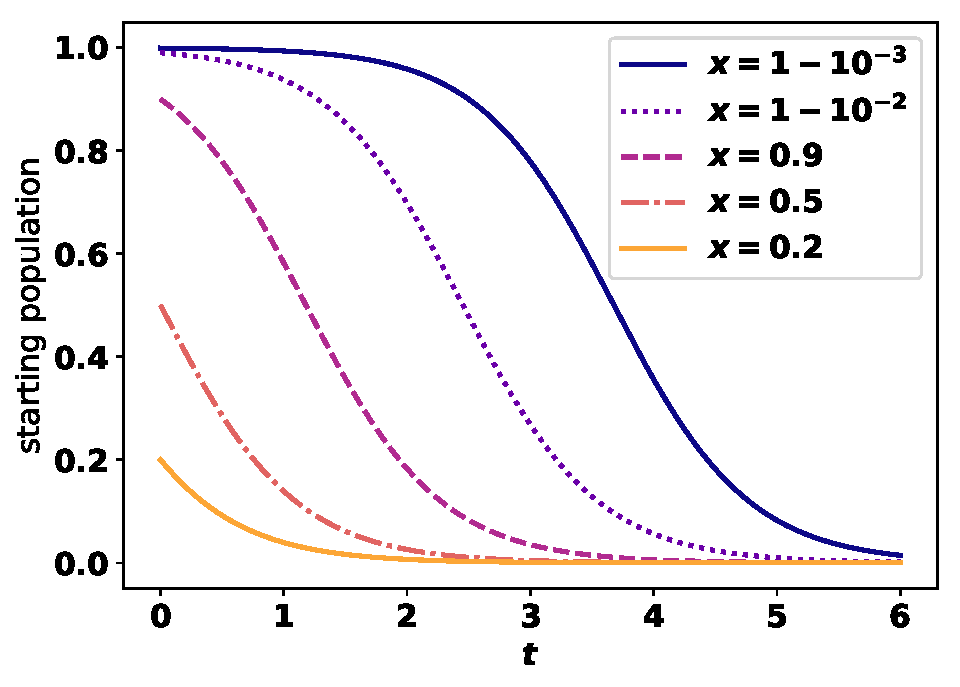
\includegraphics[width=\textwidth]{images/IndiscriminateESS-low-r.pdf}
    \caption{Low proportion of dehorned rhinos: \(r=0.05\)}
    \end{subfigure}%
    ~
    \begin{subfigure}{.3\textwidth}
    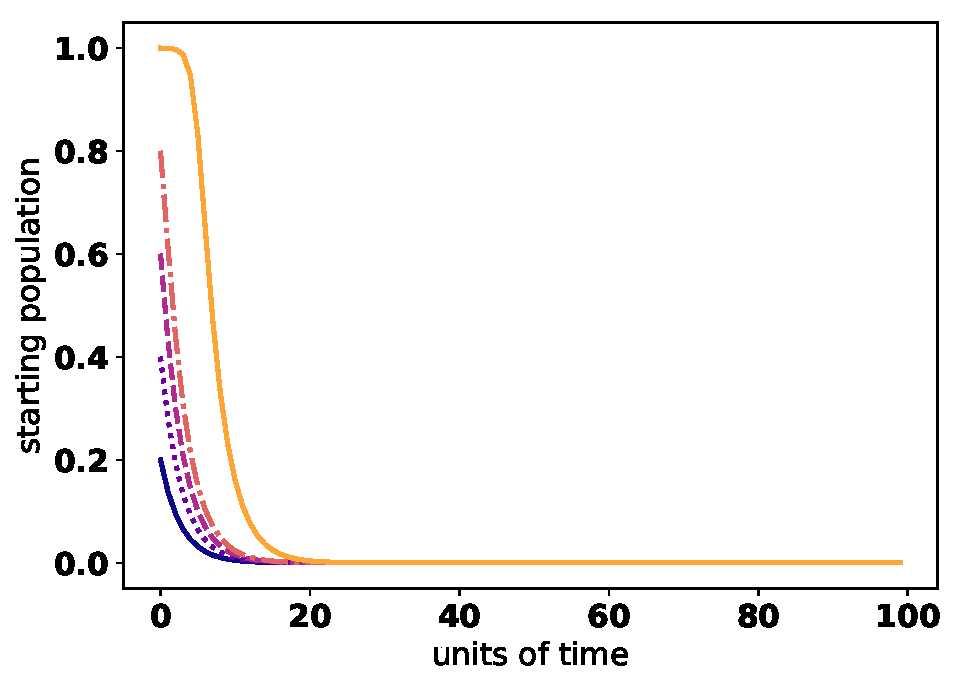
\includegraphics[width=\textwidth]{images/IndiscriminateESS.pdf}
    \caption{Majority of dehorned rhinos: \(r=0.65\)}
    \end{subfigure}%
    ~
    \begin{subfigure}{.3\textwidth}
    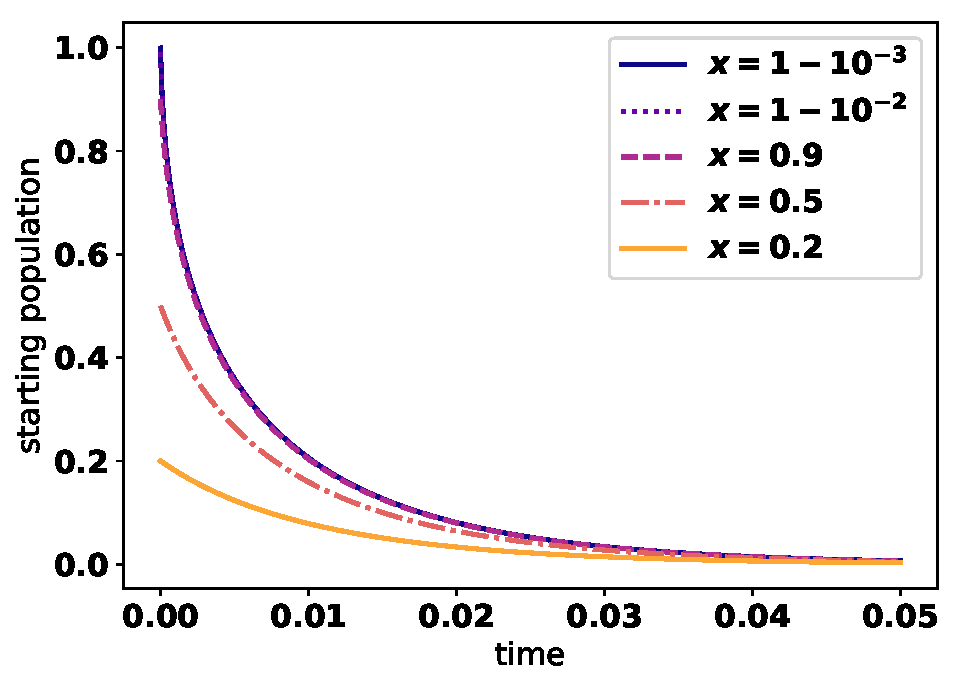
\includegraphics[width=\textwidth]{images/IndiscriminateESS-high-r.pdf}
    \caption{High proportion of dehorned rhinos: \(r=0.99\)}
    \end{subfigure}%
    \caption{\label{fig:indiscriminate_ess} The change of the population over 
    time with different starting populations. For \(F=5, H=50,  
    \alpha=2, \beta=2, \gamma=1, \theta_r=0.6\).}
\end{figure}

Poachers behaving indiscriminately is an undesirable case and these results
indicate that the life of
wild rhinos cannot be secured by dehorning. Our results disagree with the
claim of~\cite{Milner1992} that managers should dehorn
as many rhinos as possible. We believe that the resources should be 
assigned to security.

\section*{Acknowledgements}

This work was performed using the computational facilities of the Advanced
Research Computing @ Cardiff (ARCCA) Division, Cardiff University.

A variety of software libraries have been used in this work:

\begin{itemize}
    \item The Scipy library for various algorithms~\cite{scipy}.
    \item The Matplotlib library for visualisation~\cite{hunter2007matplotlib}.
    \item The SymPy library for symbolic mathematics~\cite{sympy}.
    \item The Numpy library for data manipulation~\cite{walt2011numpy}.
\end{itemize}


\bibliographystyle{plain}
\bibliography{bibliography.bib}


\end{document}
